
\chapter{Requirements Engineering}
In order to provide a functional and relevant application, it is necessary first to determine the stakeholders who influence the project in the form of a stakeholder analysis, from which a system context can then be determined. The functional and non-functional, as well as the optional requirements for the application, must then be described. A domain model can then be generated based on the information gained from all of this, which serves as a transition to database creation.

\section{Target Group and User Group}
Despite the difficulties mentioned in the introduction, the system targets both seniors and young people who would desire to have a diagnosis of their current health status situation. Given the age distribution of smartphone users today, the user base will tend to be younger but will also be used by older individuals. In Germany, 94.2 percent of people aged 14 to 19 owned a smartphone by the year 2021, according to Statista statistics. Between the ages of 20 and 29, it is 95,5 \%, and between 30 and 39, it is 96 \%. The proportion of smartphone owners among the over 70s is still around 68 percent \cite{.smartphonenutzer}.
\newline \\
One more target audience is medical professionals. The application should offer an easy-to-use interface for adding and editing data in the database, eliminating the need for technical expertise. Only the doctors' attitudes about the project can provide a more specific indication of this user group's interests. The stakeholder analysis will go into greater depth on this subject. 

\section{Stakeholder Analysis}
The first step is to identify the project's interest and demand groups. This is done through stakeholder analysis. The societal influences on the project are looked at in the stakeholder analysis. The stakeholder analysis allows for predicting variables such as "power", "interest", and potential stakeholder behavior. Stakeholders are individuals (groups), organizations, and interest groups that have the power to affect a project's success significantly. Therefore, project managers need to understand their interests and potential for influencing the project goals \cite[p. 28]{.stakeholder}. It is necessary to consider which individuals have a stake in the project's success and which individuals have the potential to influence the project in both positive and negative ways in order to identify the stakeholders. Persons affected by the project might be classified as internal or external stakeholders. 

\subsection{Internal Stakeholder}
\subsubsection{Developer}
In this project, the internal stakeholder group is relatively small. The only significant internal stakeholder will be the personification of the developer, who is also the data bank administrator. Due to the positive effects, a successful and widely used application would have on his reputation as a developer, this person has a tremendous personal interest in the project's success. The power he wields over the project is extremely high. With him, application development is not possible.
\newline \\ 
However, should the project grow, the internal stakeholders could also include personas such as project managers, physicians, etc.
\subsection{External Stakeholder}
\subsubsection{Users}
Customers, or users in the case of an application, are considered external stakeholders. They want to use a flawlessly functioning application and are keenly interested in the project's success. This can be attributed to the points mentioned in the introduction chapter. Their impact on the project appears to be significant, given that the success of an application cannot be guaranteed in the absence of a user group.
The users should be involved in the earliest stages of development to ensure that they are satisfied with the project result and subsequently use the application. This was done in the context of this work through surveys regarding the functionality wishes and preferences of the graphical user interface.

\subsubsection{Doctors}
General practitioners and specialists make up another stakeholder group. They have the option to log in to the application and change existing database entries, as well as create new entries. Their impact on the project is moderate because the internal database manager stakeholder can expand the database without them. However, the power factor can rise and improve when doctors talk to their patients about the application. A doctor's negative (or positive) impression of the initiative may deter (or pique) patients, resulting in the loss (or gain) of users. As a result, individual differences in interest in the project will also exist. One way to convince physicians of the value of the application is to visit their practices, tell them about the idea in detail, and involve them directly in the development phases. Using this way, it can be ensured that the doctors' ideas are also implemented.
\subsubsection{Stakeholder Matrix}
\begin{figure}[H]
	\centering
	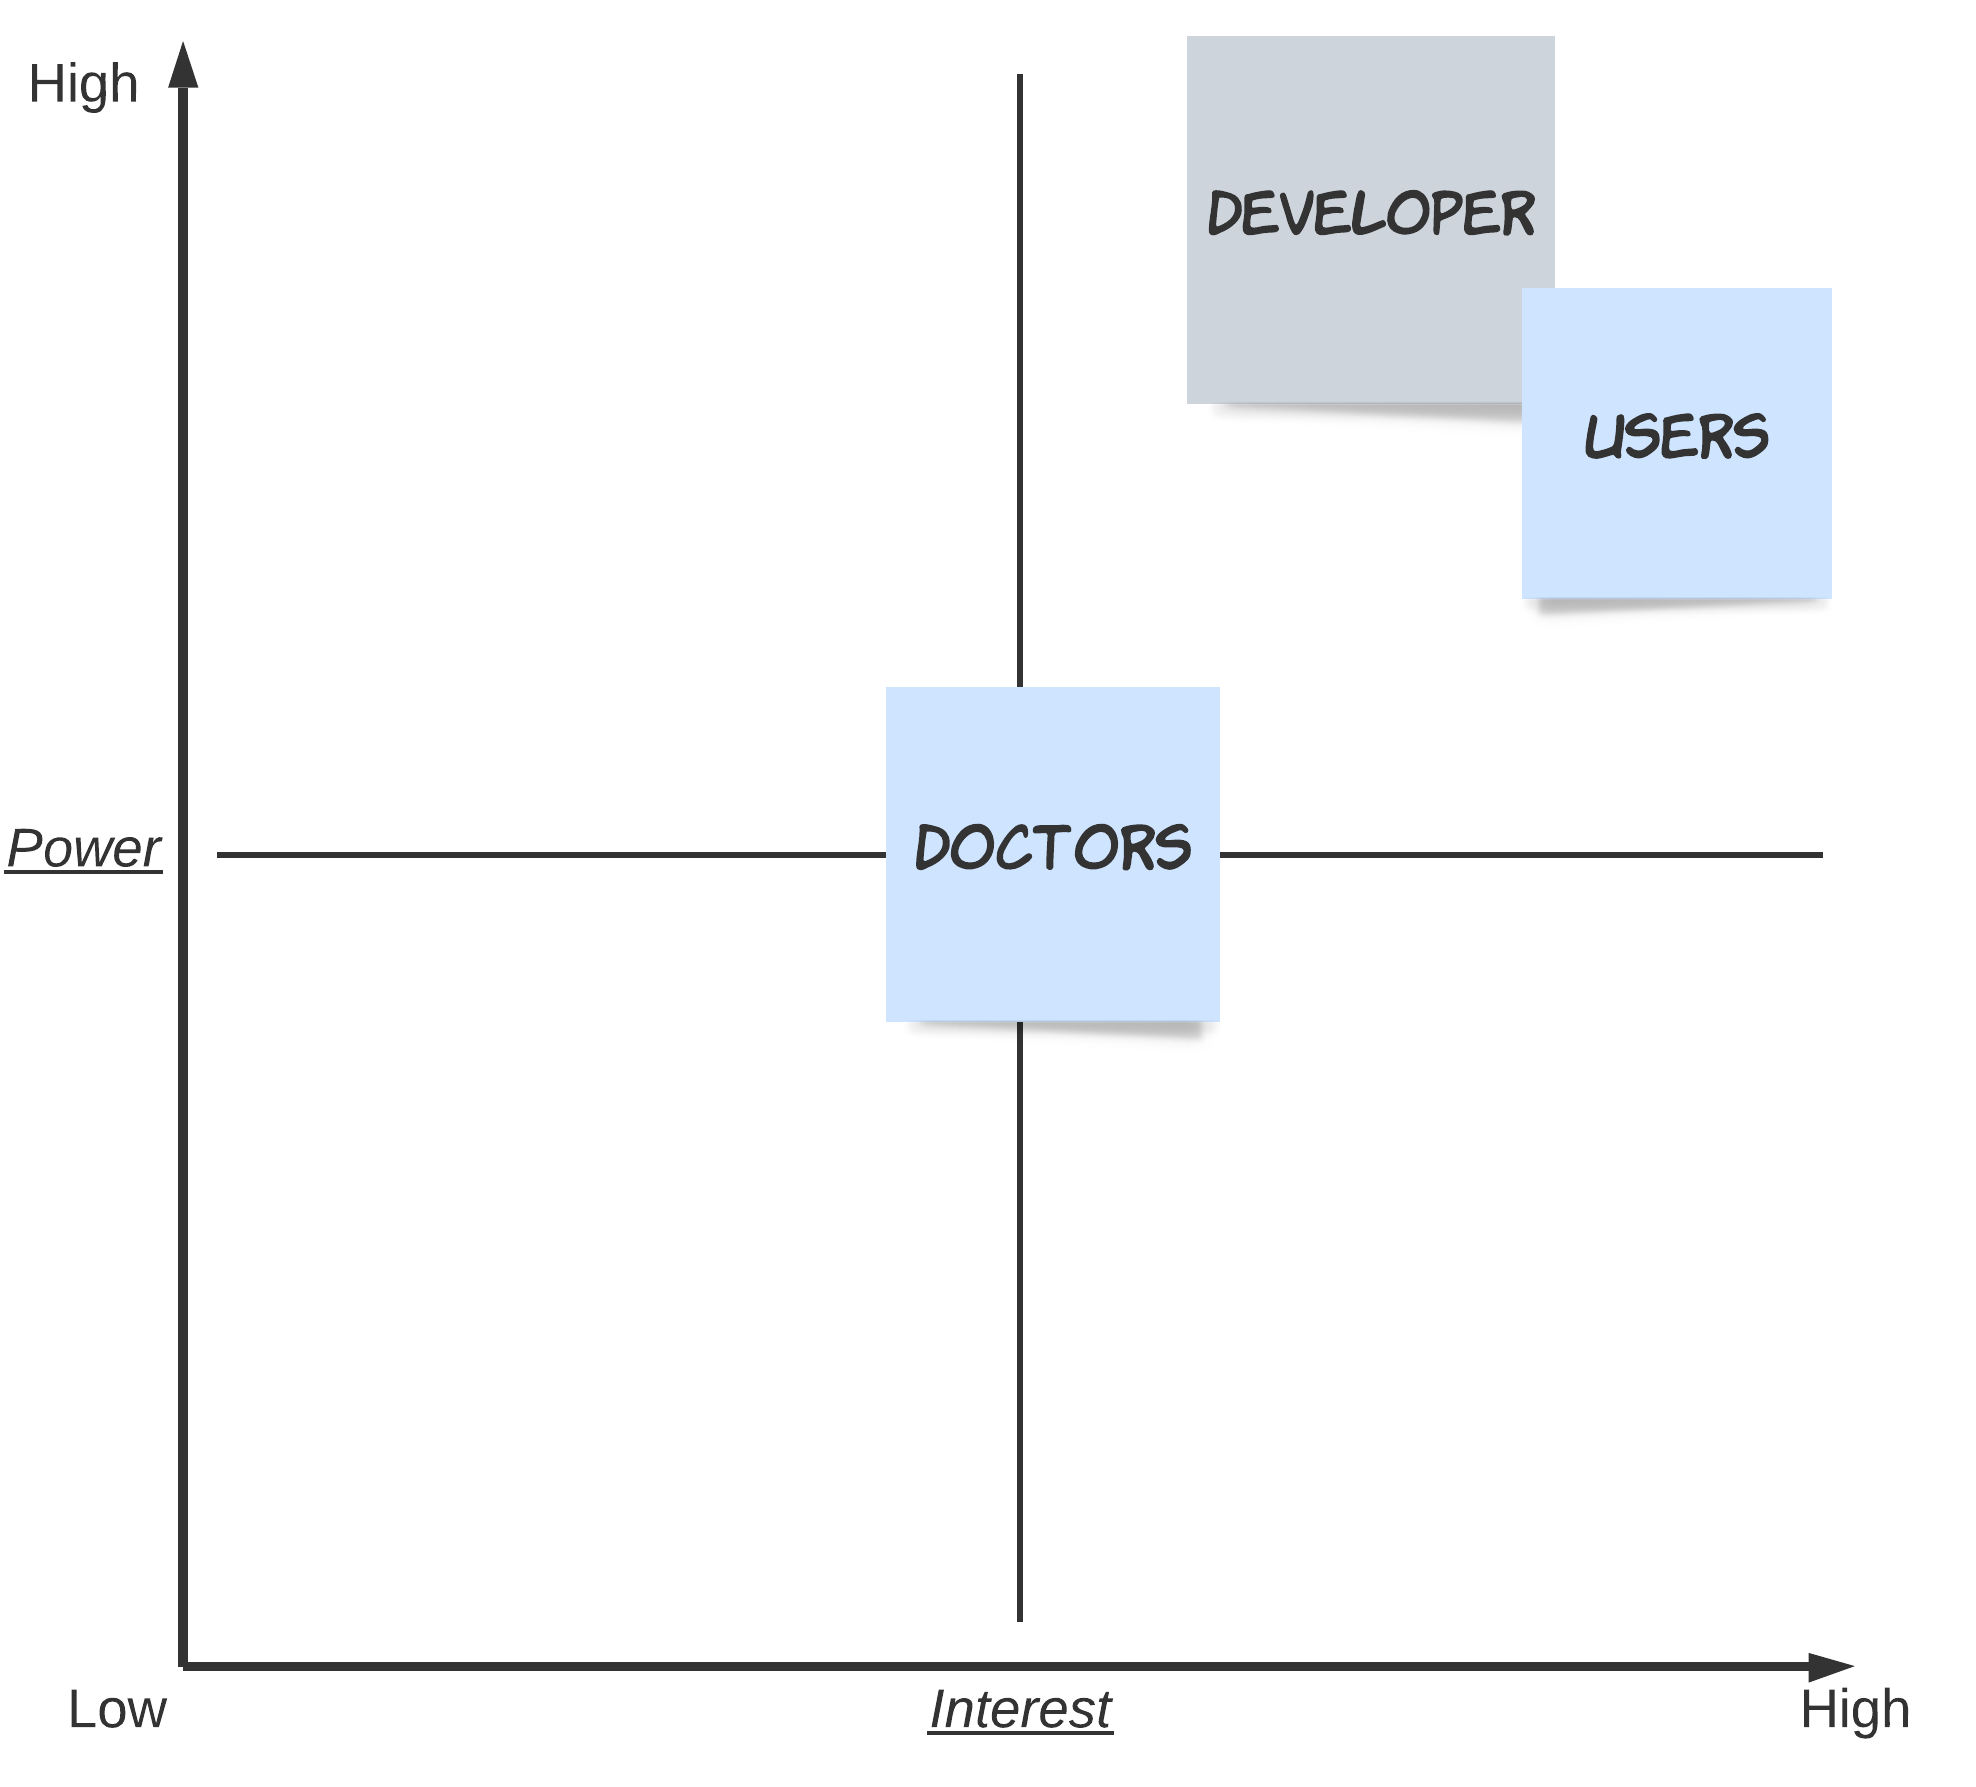
\includegraphics[scale=0.12]{stakeholder_matrix.png}
	\caption[Power/Interest Grid for Stakeholder-Analysis ]{Power/Interest Grid for Stakeholder-Analysis}
\end{figure}
\noindent	
Based on the classification of stakeholders in the matrix, the following statements can be made (based on \cite{.stakes}):
\newline \\
A close relationship should be maintained with the developer's personas and the application users. They should be allowed to give their feedback on the application, and their opinion should be considered in the development process.
\newline \\ 
Within the application doctors will also be users of the application and should be treated accordingly. However, since they cannot be categorized within the stakeholder matrix, as their impact on the project can be very different, special attention should be paid to them. This includes that they should always be satisfied so they do not bring bad words about the application to their patients. They should always be kept informed and monitored. Again, a close relationship should be maintained, and their opinion should be highly valued.

\section{System Context Diagram}
The greater environment in which a specific system or process functions is known as the system context. It covers all the outside variables and influences that affect the system's function, such as the stakeholders impacted by its operation, external systems and processes with which it interacts, and the policies and regulations it must comply with \cite{.systemcontext}. The system context can be determined using the previously performed stakeholder analysis. Determining the system context helps to understand which components interact with the system. This includes both the stakeholders and systems that influence the system.
\newline \\
The stakeholder groups of users and doctors can access the application via a smartphone. The developer and the database communicate with the system via direct code-based access. The database is filled with data from an API, and both impact the system. There are some aspects of the privacy policy and the security of the user's data, especially during the verification process of the doctors. Since, in the context of this bachelor thesis, the application will not be launched on the PlayStore, these aspects should not be addressed in the system context.

\begin{figure}[H]
	\centering
	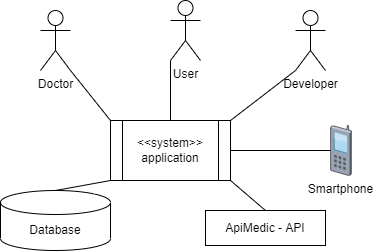
\includegraphics[scale=0.13]{system_context.png}
	\caption[System Context Diagram ]{System Context Diagram}
\end{figure}

\section{User Requirements Specification}
The requirements for an application can be divided into three categories: functional requirements, non-functional requirements, and optional requirements \cite[p. 51 ff.]{.req2} \cite{.req}. In this section, the different requirements are considered and created project-specifically. An overview of all system requirements can be found in Appendix C.

\subsection{Optional Requirements}
As the name suggests, optional requirements of an application consist of requirements that do not necessarily have to be implemented. As seen from the first survey, which can be found in Appendix A, users would like to be able to save their diagnoses. This wish forms the optional requirement 1  \textbf{([OR1])}. Another optional requirement for the system could be that a user gets the ability to save advice they browse as well - similar to the collection feature on Instagram \textbf{([OR2])}. This allows him to quickly filter and retrieve his stored advice.

\subsection{Functional Requirements}
Functional requirements are the specific capabilities, behaviors, and features that a system must have. They describe how the system must work to succeed and provide a basis for evaluating its performance and functionality. First, it should be possible for the user to switch back and forth between the different views of the application \textbf{([FR1])}. Furthermore, users shall be able to verify themselves as a doctor \textbf{([FR2]} and subsequently log in as such \textbf{([FR3])}. Once this is done, these doctors must be provided with the functionality to add new records to the database \textbf{([FR4])} and also to modify existing records \textbf{([FR5])}. Based on these records, a user should be able to start a new diagnosis \textbf{([FR6])}, which he can also save \textbf{([FR7])} and view again \textbf{([FR8])}. If the user wants to cancel the diagnosis, the system must be able to allow him to do so at any time \textbf{([FR9])}. After a diagnosis has been successfully made and saved, it must also be possible to delete the diagnosis \textbf{([FR10]1)}. Likewise, it should be possible for a doctor to cancel the addition or modification of data records at any time \textbf{([FR11])}. 


\subsection{Non-functional Requirements}
After the functional requirements have been determined, the non-functional requirements are now considered. Non-functional requirements can be described as not dealing with a user's direct interaction with the application but with the system-specific properties. This includes, for example, the reliability of the application but also safety aspects \cite{.req2}. For example, a non-functional requirement for the system is that it should be able to make correct diagnoses \textbf{([NFR1])} and do so without requiring a user to log in \textbf{([NFR2])}. In addition, the graphical interface should be intuitive for the user \textbf{([NFR3])} to ensure user-friendliness.



\section{Use Cases}
The application's architectural goal is to provide an optimal user experience for patients and doctors. In order to ensure this, it is necessary to determine, before the actual development, which uses cases the software has to cover, i.e., the externally visible interactions of the users with the system. This ensures that the application meets the users' wishes and that they use it. In addition, possible ambiguities are revealed, and required data structures are determined. Possible problems that may arise during the application use are likely to be found during the process, and technical solutions can then be worked out. Experience has shown that use cases also make it easier for a developer to create the objects that have to be created with an object-oriented programming language in the early development process more precisely and to recognize and implement inheritance options at an early stage. Some use cases can be identified from the functional and optional requirements above. Figure 3.3 shows the resulting use case diagram, which has been shortened to the most relevant use cases. 

\begin{figure}[H]
	\centering
	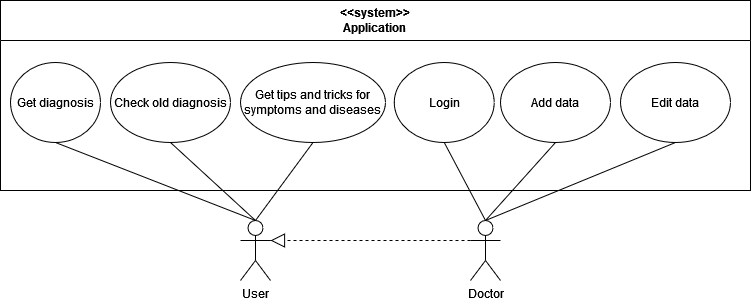
\includegraphics[scale=0.175]{use_case_diagram.png}
	\caption[Use Case Diagram]{Use Case Diagram}
\end{figure}
\noindent
The use cases are described in detail in the following sections. The resulting use case tables for each of them can be found in Appendix D.

\subsection{Get Diagnosis}
The first use case is described by the fact that a user would like to receive a diagnosis \textbf{[FR6]}. The actors who can carry out this use case are both patients, i.e., average users and doctors. In this application, doctors represent a subclass of users. In order to start the disease determination, the trigger, which will be implemented in the form of a button, must be pressed. The system then responds by displaying the view to enter and specify symptoms. As soon as the actor has finished specifying the symptoms, the system calculates the possible diseases and displays them to the actor as a diagnosis. The actor now has the opportunity to decide whether he wants to end the use case by exiting the diagnostic view or saving the diagnosis \textbf{[FR7]}, which is indicated by pressing the save button. The system then saves the diagnosis. Optionally, the actor should also be able to save the diagnosis as a PDF on his device \textbf{[OR1]}. During the process, the user can cancel the symptom statement at any time, which ends the use case by returning to the main page of the application \textbf{[FR10]}.

\subsection{Review Received Diagnoses}
After the user has received his diagnosis, he should be able to look at old diagnoses again \textbf{[FR8]}. The prerequisite for seeing such a diagnosis is that the actor had previously saved it when the diagnosis was made. A view is provided in the application in which saved diagnoses are displayed in a list. Clicking on such a diagnosis starts the use case, after which the system opens the detailed view of the diagnosis. The use case is ended by clicking on the back button provided for this purpose. While the diagnosis is being viewed, the user can delete the selected diagnosis. This is triggered by clicking on the icon provided for this purpose and is answered by deleting the diagnosis from the system. In this use case, too, the user is allowed to save his diagnosis as a PDF \textbf{[OR1]}. The procedure for this corresponds to that of the "Get Diagnosis" use case.

\subsection{Login}
As mentioned in the project goal, doctors should be allowed to log into the application \textbf{[FR3]}. The trigger for the use case is the click on the login button. Once the button is pressed, the application will display the login page. The actor can enter his credentials, at which point the system checks whether these are stored in the database. Should the result be positive, the doctor will be logged in, and the system will display the doctor's dashboard. The prerequisite for the use case to be carried out without errors is that the doctor has been able to verify himself as such beforehand \textbf{[FR2]}. If this has not yet happened, the user can click on the verify button, where he will be prompted to carry out this process and will be logged in if it is successful. Ould it is not successful because the user can not verify himself as a doctor, the system will continue showing error messages to the actor. Supposing the doctor is verified, but the system cannot find the entered credentials. In that case, the application displays an error message, and the user, suspecting that the credentials have been entered incorrectly, is asked to check his user data and try again after correcting possible input errors.

\subsection{Add Data}
Provided that he is logged in, a doctor can now add data to the database \textbf{[FR4]}. In order to do this, he must press the button provided for this purpose. The system then displays the blank template for a data record, in which the doctor can enter the data he wants to add. As soon as he has done this and pressed the confirm button, the system adds the data record to the database and saves it in his data list. Suppose the actor presses the confirm button without entering anything in each data field. In that case, the application will display an error notification on the screen, prompting the user to fill in all data fields. If the user wishes to cancel the process, he is free to press the button provided for this at any time, after which the system closes the view, and the use case ends \textbf{[FR11]}. 

\subsection{Edit Data}
In addition to the functionality to create new datasets, the doctor should be able to expand and edit existing datasets \textbf{[FR5]}. The structure of this use case is similar to the previously described use case of adding new data. The doctor must first be in the view where all existing data records are displayed in list format. There he has the opportunity to click on one of these data sets, which signals to the system that it must now display the editing screen for the selected data set. In this view, the doctor can make the desired changes and press the confirm button. The application will then update the record in the database, and the use case will be terminated. As before, when adding new data records, the doctor can end the process at any time \textbf{[FR11]}.

\subsection{Get Tips and Tricks for Symptoms and Diseases}
The final use case worth mentioning is viewing advice on illnesses \textbf{[FR1]}. A user can go to the view for all advice that Doctors have uploaded. Once he has navigated there and the system shows the predicted view, he can click on one of the pieces of advice there, which will be shown to him in detail afterward. Optionally, the user can save the advice as a favorite by clicking on the button provided for this purpose \textbf{[OR2]}. 

\section{Domain Model}
Domain modeling is a vital modeling topic in Agile development at scale because there is frequently a gap between comprehending the issue domain and interpreting requirements. It depicts the solution as a collection of domain objects that collaborate to satisfy system-level scenarios \cite{.safe}. The quintessence of the object-oriented analysis step is decomposing a domain into problem-relevant concepts or objects. A domain model is a visual representation of the problem-relevant domain classes of a domain \cite{.safe}. With the help of unified modeling language (UML) notation, a domain model is represented by a set of class diagrams defined \cite{.domainmodel}. They usually consist of no methods or functions. It presents a conceptual perspective and can show domain objects or classes, as well as associations between domain classes and attributes of domain classes \cite{.safe} \cite{.domainmodel}. Identifying domain entities and their connections, derived from a grasp of system-level requirements, offers a good foundation for understanding and supports practitioners in designing systems for maintainability, testability, and incremental development \cite{.safe}. Finding conceptual classes by recognizing substantive phrases is an effective technique for domain modeling \cite[p. 76]{.domainmodel}.

\begin{itemize}
	\item A person is a \textbf{user} of the application.
	\item A \textbf{user} chooses a \textbf{body part}.
	\begin{itemize}
		\item A \textbf{body part} can be associated with different \textbf{symptoms}.
		\item A \textbf{user} selects a \textbf{symptom} and specifies the selected symptom by narrowing down (selecting) \textbf{proposed symptoms}, the \textbf{time of occurrence} and the \textbf{symptom intensity}. The information obtained is summarized as a textbf{user-specified symptom}.
	\end{itemize}
	\item One or more \textbf{user-specified symptoms} lead to the calculation of one or more possible \textbf{diseases}.
	\begin{itemize}
		\item A \textbf{disease} has different \textbf{symptoms}.
	\end{itemize}
	\item A \textbf{diagnosis} consists of one or more \textbf{diseases}.
	\item \textbf{Doctors} are special \textbf{users} of the application.
	\item \textbf{Doctors} can add/edit \textbf{advices}, \textbf{symptoms}, \textbf{body parts} and \textbf{diseases}.
	\item \textbf{Users} can view \textbf{advices}.  
\end{itemize}
\noindent
The information just obtained makes it easier to create the domain model. The entities user, symptom, user-specified symptom, body part, diseases, doctor, advice, and diagnosis, can already be recognized. Based on that information, a domain model can be created. 
\begin{figure}[H]
	\centering
	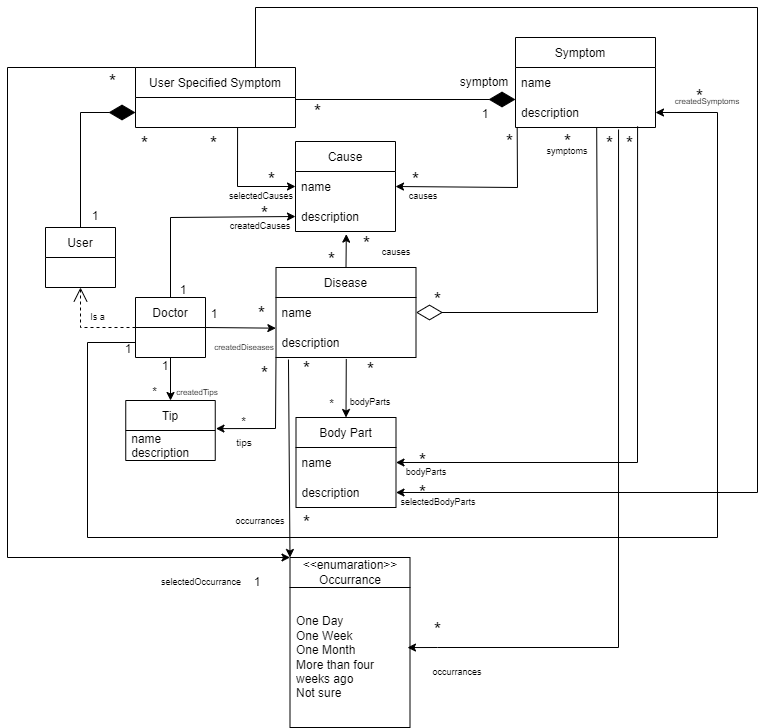
\includegraphics[scale=0.225]{domain_model.png}
	\caption[Domain Model]{Domain Model}
\end{figure}
\noindent
Based on the domain model and the previously obtained information, database development can now be started. Later on, the chapter optimizations also address some aspects that have been neglected.

